% using Elseveir template per https://www.elsevier.com/authors/author-schemas/latex-instructions
% model paper: Dynamic effects of teacher turnover on the quality of instruction (2016)
%   from Economics of Education Review
\documentclass[review]{elsarticle}

\usepackage{lineno,hyperref}
\modulolinenumbers[5]

\journal{Journal of \LaTeX\ Templates}
\bibliographystyle{elsarticle-num}
\usepackage{booktabs}
\usepackage{graphicx}
\graphicspath{{../alt-ed-survey/figures-and-tables}}
\usepackage{hyperref}
\usepackage{threeparttable}  
\usepackage{tikz}
\usetikzlibrary{calc,matrix}

\begin{document}

\begin{frontmatter}

\title{
    Dynamic Effects of H-1B and Section 127 Policy Interaction on Higher Education
    \tnoteref{titlenotes}
}
% \tnotetext[titlenotes]{
%     Go to \url{https://github.com/Vandivier/research-dissertation-case-for-alt-ed/tree/master/papers/}
%     for additional materials including the online appendix,
%     survey data, and data analysis source code.
% }

\author[mymainaddress]{John Vandivier} % \fnref{authorlinefootnote}}
\address[mymainaddress]{4400 University Dr, Fairfax, VA 22030}
\ead{jvandivi@masonlive.gmu.edu}



\begin{abstract}
    % It is widely believed that teacher turnover adversely affects the quality of instruction in urban schools serving predominantly disadvantaged children,
    % and a growing body of research investigates various components of turnover effects.
    % The evidence at first seems contradictory,
    as the quality of instruction appears to decline following turnover despite the fact that most work shows higher attrition for less effective teachers.
    This raises concerns that confounding factors bias estimates of transition differences in teacher effectiveness,
    the adverse effects of turnover or both.
    % After taking more extensive steps to account for nonrandom sorting of students into classrooms and endogenous teacher exits and grade-switching,
    % we replicate existing findings of adverse selection out of schools and negative effects of turnover in lower-achievement schools.
    But we find that these turnover effects can be fully accounted for by the resulting loss in experience and productivity loss following the reallocation of some incumbent teachers to different grades.

    It is widely believed that employer educational assistance increases the quantity demanded for higher education,
    but the original passage of Section 127 which enables this tax-deduction for employers is associated with a reduction to the growth of higher education enrollment.
    Comparative supply-side and demand-side explanations are discussed and evaluated.
    After taking extensive steps to account for policy and other changes in the economy,
    real variation in employer educational assistance over time is exploited
    to identify the effect of the employer assistance amount on higher education enrolment using Dynamic Ordinary Least Squares (DOLS).
    We robustly identify a positive effect on enrollment from employer educational assistance.
    % what is the coefficient? mention vector autoregression too
    However X
    Therefore Y

    % Highlights
    % 1. Section 127 Employer Assistance
    % 2. 
    % 3. 
    % 4. 
    
    % degree requirement as a strategy to import cheap, effective foreign labor (VISA)
    % this prevents high school graduates from directly entering roles that typically award section 127 (white color, major employer, corporate work)
    % until recently, that is, with walmart, mcdonalds, starbucks giving section 127 i think even to part timers
    % 1952 allows unlimited merit immigration, 1990 there is a quota and degree requirement added to H-1B: https://en.wikipedia.org/wiki/H-1B_visa#Immigration_Act_of_1990
    % New and initial H-1B and H-1B1 visas issued by the U.S. Department of State through consular offices
    % https://en.wikipedia.org/wiki/H-1B_visa#H-1B_visas_issued_per_year
    % crackdown in 2017: https://www.investopedia.com/news/impact-trumps-h1b-visa-crackdown-5-charts/
    % Theory: After 1990, companies began requiring a 4 year degree so they could have an H-1B justification.
    % This caused more americans to pursue an undergraduate degree without section 127. we should see section 127 use decline after 1990.
    % Recently, employers have begun giving the benefit anyway due to labor selection and internal ROI benefits
\end{abstract}

\begin{keyword}
education economics, section 127, educational assistance, gi bill, h-1b, debt crisis, dols
\MSC[2010] % TODO
\end{keyword}

\end{frontmatter}

\pagebreak
\linenumbers
        
    \section{Introduction}

    Basic supply and demand theory indicate that a reduction in price is associated with an increase to the quantity demanded.
    In 1978, employer educational assistance became tax-deductable in the United States up to the original, nominal limit of 5,000 dollars.
    It is surprising, therefore, that 1978 is associated with a local decrease in the growth rate on both total and public university enrollment.
    This study exploits real variation in the tax-deductable employer educational assistance limit to eventually identify the expected positive effect,
    but not before identifying and correcting for several interesting things going on in the economy.
    Specifically, an interaction between H-1B policy and Section 127 employer educational assistance is discovered and assessed.

    \subsection{Supply-Side Explanations}
    Before forming more exotic theories, some simpler hypotheses should be checked.
    One hypothesis is that there is an adjustment period after the passage of Section 127 and before widespread employer provision of the newly deductable benefit.
    Allowing for a 3 or 5 year lag around the passage of Section 127 in 1978 does not resolve the issue.
    Across the eight five-year periods from 1970 to 2010, the five-year public enrollment growth rate was above 9 percent as often as it was below.
    Two of the four low-rate intervals occured immediately subsequent to the 1978 creation of Section 127.
    The interval just prior, from 1970-1975, saw the highest growth in enrollment across the period.
    It does not appear to be a one-year fluke that the employer educational assistance is associated with declined enrollment growth.

    An alternative to the 3 or 5 year lagged analysis is to directly refer to surveys of employers.
    Cappelli\cite{cappelli2004employers} identifies 3 employer surveys from 1992 and 1993 which indicate that at least 86 percent of surveyed employers provided educational assistance.
    These studies were samples of convenience with a focus on large employers,
    but additional information leads Cappelli to claim that a substantial majority of employers offer such plans over his period of analysis from about 1990 to 2004.
    Cappelli notes that employee utilization of the benefit favors graduate education
    with about 20 percent of graduate students receiving employer assistance
    and roughly 6 percent of undergraduates doing so.
    Common provision of the benefit has remained true in later years.
    In 2013, SHRM reported that 61 percent of employers offer tuition assistance\cite{cherry2014rejuvenating}.
    In 2017, World at Work found that 85 percent of employers offered such a benefit,
    with another 7 percent offering non-reimbursement tuition assistance, such as upfront tuition discounts\cite{talentculture_2018}.

    \subsection{H-1B, GI Bill, and Stafford Loan Connections}
    The idea that graduate students mainly use employer education benefits motivates hypotheses around undergraduate access.
    Increasingly since the 1990s, developed economies have experienced degree inflation and experience inflation.
    Entry level positions now require a degree when previously this was not necessary, even when technology has made the work easier.
    It is possible that undergraduate access to employer benefits are reduced simply because employers increasingly hire individuals that already have the degree.
    Employers are known to value the degree as a signal of labor quality, but these days there are plenty of other, richer data sources on quality for certain professions.
    In computer programming we see some employers completely dropping the degree requirement and preferring technical interviews, digital portfolio evaluation, and other signals.
    Why, then, do other leading employers continue to require the degree?
    One answer is that the degree requirement forms an H-1B justification.
    Since the passage of the Immigration Act of 1990\cite{law1990law}, a corporation must claim a shortage of qualified specialized labor to justify an H-1B.
    The "attainment of a bachelor's or higher degree" is written into the law as a test of whether labor is qualified and specialized.
    This would motivate employers to begin requiring the degree in order to obtain cheap immigrant labor, even while knowing the degree may not be necessary.

    Zero employers offered Section 127 educational assistance in 1977, but the majority offered the benefit by 1993.
    Immigration policy is a change which interrupts this period of analysis, but there are two other major policies to take note of.
    Stafford loans were available before Section 127, but the limits and rules for these loans and other government assistance to higher education fluctuated over the period of analysis.
    Government educational benefits for veterans is another major policy in the higher education assistance space.
    It becomes difficult to imagine a proper Section 127 analysis which does not include dynamic correction for these potentially important factors,
    as well as correction for general price changes and economic conditions in the economy over time.
    Such a corrected analysis is exactly what this paper completes.

    \subsection{Demand-Side Explanations}
    The prior explanations consistitute a supply-side exploration of the impotence of Section 127.
    An alternative explanation is that there simply wasn't much demand for college in the early years of Section 127.
    Indeed, lack of market demand appears to be a good explanation for the consistent college-age enrollment percent
    which is observed at 25.7 percent in both 1970 and 1980.
    A demand-side explanation is consistent with the falling average tuition and fees observed for all institutions from 1972 to 1980.
    After 1980 we see an upward trend in price and also an upward trend in college-age enrollment percentage, as well as simple total enrollment.

    With an increase to the Stafford limit in the 1977 school year,
    a major change to the GI Bill in the 1981 school year,
    Section 127 beginning in the 1978 school year,
    and price changes in higher education and for all other goods,
    claims about a particular cause become dubious without full and corrective statistical treatment.
    Even so,
    there is some plausibility to the claim that Section 127 was passed during a time when demand was weak,
    so that there may have been a positive effect on the part of Section 127 as early as the first year,
    but it was overshadowed by general decline.
    The main contribution of this line of thought to a more general analysis is that corrective statistics should include price data
    for education in particular, and also for the general economy.

    % \section{Texas Schools Project data}
    \section{Data}

    % \section{Teacher transitions and productivity}
    \section{Empirical Model}

    % \section{Aggregate disruption}
    \section{Aggregate Results}

    % \section{Reconciling selection and turnover effects in low-achievement schools}
    % \section{Reconciling selection and turnover effects in low-achievement schools}

    \section{Conclusions}

        % maybe talk about stress and debt for why debt is important

        % NPSAS:19
        % Average undergraduate tuition and fees
        % for full-time students in all degree-granting postsecondary institutions,
        % by level and control of institution: Selected years, 1970-2016 [school year beginning 2016]
        % https://nces.ed.gov/programs/digest/d17/tables/dt17_330.10.asp
        % Constant 2016 dollars

        % inflation adjustment by PCE over time
        % https://fred.stlouisfed.org/series/PCE

        % 2016 is base year for corrected real deduction limit

        % Percentage of 18- to 24-year-olds enrolled in college,
        % by level of institution and sex and race/ethnicity of student: 1970 through 2017
        % https://nces.ed.gov/programs/digest/d18/tables/dt18_302.60.asp

        % college more diverse than ever https://www.aacu.org/aacu-news/newsletter/2019/march/facts-figures
        % more poor folks entering college https://www.insidehighered.com/news/2019/05/23/pew-study-finds-more-poor-students-attending-college
        % but can we do even better...? and not saddle them with debt? are these folks more in debt (higher debt load by status)...?
        
        % total enrollment: https://nces.ed.gov/programs/digest/d18/tables/dt18_303.10.asp

        % what about student loans? here are the limits over time: https://www.finaid.org/loans/historicallimits.phtml
        % actual undergrad loans awarded since 1990 in the excel at https://research.collegeboard.org/trends/student-aid
        % My variable `Total UG Federal Loans` adapted from CB xlsx worksheet `Table 2_UG`
        % but i don't think we should use actuals there bc that would explain away demand effects...we want to preserve those (do a better job explaining this plz)
        % so, prefer the limits over time...those are attributed to the school year, so rules beginning July 1993 are true for 1993 (start of school year)
        % eg dummy for "limit is subsidized plus unsubsidized" begins to be true for 1993 in my csv
        %
        % GI Bill accounting https://en.wikipedia.org/wiki/G.I._Bill#Chapter_30_(Montgomery_GI_Bill)
        % Variable implemented as categorical
        % [state A] original bill was 1944-1984
        % [state B] VEAP established 1981 https://www.benefits.va.gov/gibill/veap.asp
        % [state C] Montgommery GI went into effect 1984
        % [state D] Post-9/11 Montgomery GI Bill went into effect for 2009 school year https://www.thebalancecareers.com/gi-bill-for-the-21st-century-3347143
        % [state E] Forever GI bill rolls out new benefits starting in 2018 https://rebootcamp.militarytimes.com/education-transition/education/2017/08/16/trump-signed-the-forever-gi-bill-here-are-11-things-you-should-know/

        \section{Results}
        
        % \begin{table}
        %     \caption{Medium and Strong Models, Selected Variables}
        %     \begin{tabular}{lllll}
        %     Factor & 2018 Medium & 2018 Strong & 2019 Medium & 2019 Strong \\
        %     \toprule
        %     Male &  &  & -2.458* & -0.422** \\
        %     Not STEM & -1.269* \\
        %     X$_0$ & 1105.125 & .106 & -12345.347* & 3.289*** \\
        %     \bottomrule
        %     R-Squared & .597 & .504 & .526 & .319 %
        
        %     \end{tabular}
        %     \begin{tablenotes}
        %         \item{
        %             * p $<$ .05
        %             ** p $<$ .01
        %             *** p $<$ .001
        %         }
        %     \end{tablenotes}
        %     \label{tab:models}
        %     \end{table}
        
        % \begin{figure}[h!]
        %     \centering
        %     \caption{Employer Driven Favorability}
        
        %     \begin{tikzpicture}[element/.style={minimum width=1cm, minimum height=0.75cm}]
        
        %     \node (n1) [above=0.25cm] {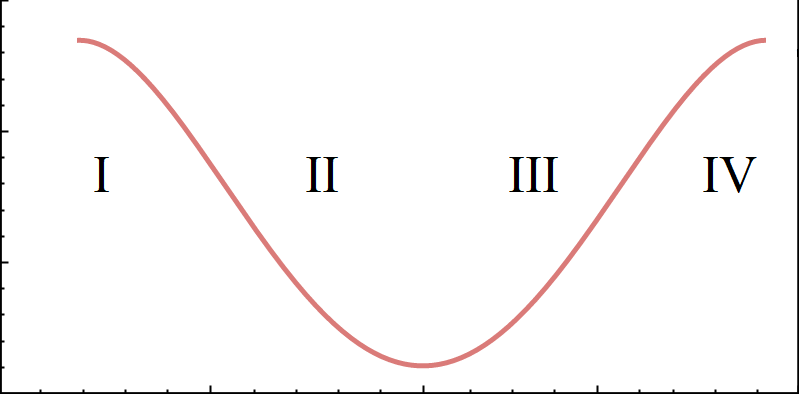
\includegraphics[width=0.5\textwidth]{../alt-ed-survey/figures-and-tables/figure-4.png}};
        %     \node (n2) [above=0.25cm] at ($(n1)!0.5!(n1) - (4, 1)$) {\rotatebox{90}{\textbf{Suitability}}};
        %     \node (n3) [above=0.25cm] at ($(n1)!0.5!(n1) - (0, 3)$) {\textbf{Time}};
        
        %     \end{tikzpicture}

        %     \label{fig:employer_driven_favorability}
        %     \end{figure}

        \section{Conclusions}
        
        % Pub. L. 99–514, § 1162(a)(2), substituted “$5,250” for “$5,000” in heading and twice in text
        % https://www.law.cornell.edu/rio/citation/Pub._L._99-514
        % https://www.ucop.edu/research-policy-analysis-coordination/_files/Public%20Law%2099-514.pdf
        % it moved 5000->5250 in 1986
        % can we see effect on median-and-below vs above?
        % important to look at wages not income (which would include investments, etc, see shrm's discussion: http://www.cpepea.com/wp-content/uploads/2017/05/10-0418-Coalition-Report-on-Public-Policy-Issue-E-P-E-A_FNL.pdf)
        % SHRM assessed only a single year, 2008. Shows Section 127 is mostly a Master's degree tool rn.
        % 75 percentile for salaries in 2017 was 54250 https://bizfluent.com/info-10032733-percentile-salary.html
        % define middle class as 50-75 percentile, lower class as under 50 percentile. break down effect by salary classification and see if it helps lower/middle
        % if so, it should improve diversity of education leading to a more diverse workforce which employers crave (TM) and politicians, etc...
        % Should we actually enact this policy? Effect on alternative credentials and credential inflation
        % Other options like extending the benefit to repayment https://blog.shrm.org/blog/let-s-fight-the-skills-gap-by-expanding-tax-free-education-assistance
        % we can also consider extending the education benefit to unaccredited education and income share agreements not just loans
        
        % https://www.nber.org/papers/w9225.pdf 
        % https://www.nber.org/digest/feb03/w9225.html

        \bibliography{./BibFile}
        
        \end{document}
        